\documentclass[10pt]{beamer}

% ------------------------------------------------------------------------
% Carga del preámbulo personalizado (preamble.tex)
% ------------------------------------------------------------------------
\usetheme[progressbar=frametitle]{metropolis}
\usepackage{appendixnumberbeamer}
\usepackage{fancyvrb}
\usepackage{booktabs}
\usepackage[scale=2]{ccicons}
\usepackage{pgfplots}
\usepgfplotslibrary{dateplot}
\usepackage{type1cm}
\usepackage{lettrine}
\usepackage{ragged2e}
\usepackage{xspace}
\newcommand{\themename}{\textbf{\textsc{metropolis}}\xspace}
\usepackage{graphicx} % Allows including images
\usepackage{booktabs} % Allows the use of \toprule, \midrule and \bottomrule in tables
\usepackage[utf8]{inputenc} %solucion del problema de los acentos.
\usepackage{xcolor}
\definecolor{LightGray}{gray}{0.9}

\usepackage{minted}
\usemintedstyle{tango}
\newcommand{\mypyfile}[1]{\inputminted[linenos=true, fontsize=\footnotesize, frame=lines, framesep=5\fboxrule,framerule=1pt]{python}{#1}}

\setminted[python]{breaklines,frame=lines,framesep=2mm,baselinestretch=1.2,bgcolor=LightGray,linenos, fontsize=\footnotesize} % obeytabs=true, tabsize=2, showtabs=true}

%%%%%%%%%%%%%%%%%%%%%%%%%%%%%%%%%%%%%%%%%%%%%%%%%%%%%%%%%%%%%%%%%%%%%%%%%%%%%%%%%%%%%%
\setbeamercolor{progress bar}{fg=blue!50!black,bg=white!50!black}
\setbeamercolor{title separator}{fg=red!50!black,bg=white!50!black}
\setbeamercolor{frametitle}{fg=white!80!black,bg=red!50!black}
\title[PCFI161]{Programaci\'on para F\'isica y Astronom\'ia}
\subtitle{Departamento de Física.}

\newcommand{\myfront}{
\author[PCFI161]{Corodinadora: C Loyola \\ Profesoras/es C Loyola / C Femenías / Y Navarrete / C Ruiz}
\institute[UNAB]{Universidad Andrés Bello}
\date{Primer Semestre 2025}
}

\titlegraphic{%
  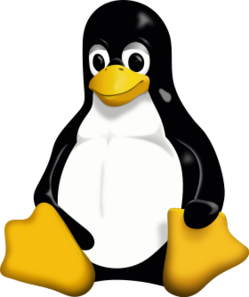
\includegraphics[width=.08\textwidth]{logo-tux.png}\hfill
  
\includegraphics[width=.3\textwidth]{logo-unab.png}\hfill
  
\includegraphics[width=.08\textwidth]{logo-python.png}
}

\makeatletter
\setbeamertemplate{title page}{
  \begin{minipage}[b][\paperheight]{\textwidth}
    \vfill%
    \ifx\inserttitle\@empty\else\usebeamertemplate*{title}\fi
    \ifx\insertsubtitle\@empty\else\usebeamertemplate*{subtitle}\fi
    \usebeamertemplate*{title separator}
    \ifx\beamer@shortauthor\@empty\else\usebeamertemplate*{author}\fi
    \ifx\insertdate\@empty\else\usebeamertemplate*{date}\fi
    \ifx\insertinstitute\@empty\else\usebeamertemplate*{institute}\fi
    \vfill
    \ifx\inserttitlegraphic\@empty\else\inserttitlegraphic\fi
    \vspace*{1cm}
  \end{minipage}
}
\makeatother


\makeatletter
\setlength{\metropolis@titleseparator@linewidth}{2pt}
\setlength{\metropolis@progressonsectionpage@linewidth}{2pt}
\setlength{\metropolis@progressinheadfoot@linewidth}{2pt}
\makeatother


\begin{document}

% ------------------------------------------------------------------------
% Portada
% ------------------------------------------------------------------------
\myfront{
  \title{Repaso Integral y Actividades Complementarias}
  \subtitle{Segunda Clase de Repaso}
  \date{31 de Marzo 2025}
}

% ------------------------------------------------------------------------
% Slide 1: Título de la Sesión
% ------------------------------------------------------------------------
\begin{frame}
  \titlepage
\end{frame}

% ------------------------------------------------------------------------
% Slide 2: Índice / Tabla de Contenidos
% ------------------------------------------------------------------------
\begin{frame}
  \frametitle{Índice}
  \tableofcontents
\end{frame}

% ----------------------------------------------------------------------------------------
% SECCIÓN 1: Introducción y Objetivos
% ----------------------------------------------------------------------------------------
\section{Introducción y Objetivos}

\begin{frame}{Objetivos de la Sesión de Repaso}
  \begin{itemize}
    \item Revisar y consolidar los contenidos previos (Unidades I a IV).
    \item Resolver dudas y reforzar conceptos fundamentales: sintaxis, estructuras de control, funciones, módulos y uso de librerías.
    \item Desarrollar actividades interactivas y colaborativas que estimulen el pensamiento algorítmico.
    \item Practicar mediante ejercicios de opción múltiple y programas entretenidos que integren los conceptos aprendidos.
  \end{itemize}
\end{frame}

% ----------------------------------------------------------------------------------------
% SECCIÓN 2: Repaso de Contenidos Clave
% ----------------------------------------------------------------------------------------
\section{Repaso de Contenidos Clave}

\begin{frame}{Resumen de Unidades y Conceptos}
  \begin{itemize}
    \item \textbf{Elementos Básicos} \\ 
      Diseño de programas, uso de GNU/Linux, Google Colab y el intérprete Python.
    \item \textbf{Programación en Python} \\ 
      Tipos de datos, operaciones, manejo de ficheros, funciones, paquetes y módulos.
    \item \textbf{Iteradores} \\ 
      Uso de bucles (\texttt{while} y \texttt{for}).
    \item \textbf{Funciones} \\ 
      Implementación de funciones.
  \end{itemize}
\end{frame}

% ----------------------------------------------------------------------------------------
% SECCIÓN 3: Actividades Interactivas y de Repaso
% ----------------------------------------------------------------------------------------
\section{Actividades de Repaso}

\subsection{Preguntas de Alternativas}
\begin{frame}{Ejercicio: Preguntas de Alternativas}
  A continuación se presentan algunas preguntas de opción múltiple para autoevaluar conocimientos:
  \begin{enumerate}
    \item ¿Cuál es el propósito principal de utilizar funciones en Python?
      \begin{enumerate}[A)]
        \item Facilitar la lectura y reutilización del código.
        \item Incrementar la velocidad de ejecución del programa.
        \item Permitir la interacción con bases de datos.
        \item Aumentar la complejidad del código.
      \end{enumerate}
    \item ¿Qué operador se utiliza para multiplicar en Python?
      \begin{enumerate}[A)]
        \item \texttt{/}
        \item \texttt{x}
        \item \texttt{\%}
        \item \texttt{*}
      \end{enumerate}
  \end{enumerate}
  \vspace{0.3cm}
\end{frame}



\begin{frame}{Ejercicio: Preguntas de Alternativas - Elementos Básicos y GNU/Linux} 
    \begin{enumerate} 
        \item ¿Cuál de los siguientes es un componente esencial de un sistema operativo GNU/Linux? 
        \begin{enumerate}[A)] 
            \item El kernel. 
            \item La aplicación de ofimática. 
            \item El navegador web. 
            \item El entorno de escritorio exclusivo. 
        \end{enumerate} 
        \item ¿Qué ventaja ofrece Google Colab para quienes inician en la programación? 
        \begin{enumerate}[A)] 
            \item Permite acceder a recursos computacionales gratuitos en la nube. 
            \item Requiere la instalación local de paquetes costosos. 
            \item Solo funciona con el intérprete de C++. 
            \item No permite compartir el código entre usuarios. 
        \end{enumerate} 
    \end{enumerate} 
\end{frame}

\begin{frame}{Ejercicio: Preguntas de Alternativas - Programación en Python: Tipos de Datos} 
    \begin{enumerate} 
        \item ¿Cuál de los siguientes tipos de datos no existe en python? 
        \begin{enumerate}[A)] 
            \item int
            \item float
            \item fractal 
            \item complex 
        \end{enumerate} 
        \item ¿Qué función se utiliza para determinar el tipo de dato de una variable en Python? 
        \begin{enumerate}[A)] 
            \item type(). 
            \item int(). 
            \item str(). 
            \item print(). 
        \end{enumerate} 
    \end{enumerate}
\end{frame}

\begin{frame}{Ejercicio: Preguntas de Alternativas - Programación en Python: Operaciones y Funciones} 
    \begin{enumerate} 
        \item ¿Cuál es el operador de potenciación en Python? 
        \begin{enumerate}[A)] 
            \item \texttt{*} 
            \item \texttt{**} 
            \item \texttt{$\wedge$} 
            \item \texttt{//} 
        \end{enumerate} 
        \item ¿Qué función se utiliza para convertir un número flotante a entero? 
        \begin{enumerate}[A)] 
            \item int(). 
            \item float(). 
            \item str(). 
            \item bool(). 
        \end{enumerate} 
    \end{enumerate}
\end{frame}

\begin{frame}{Ejercicio: Preguntas de Alternativas - Funciones: Conceptos Básicos} 
    \begin{enumerate} 
        \item ¿Cuál es la principal finalidad de utilizar funciones en Python? 
        \begin{enumerate}[A)] 
            \item Reutilizar y organizar el código. 
            \item Incrementar la complejidad del programa. 
            \item Reducir la legibilidad del código. 
            \item Evitar el uso de módulos externos. 
        \end{enumerate} 
        \item ¿Cómo se define una función en Python? 
        \begin{enumerate}[A)] 
            \item Con la palabra reservada \texttt{function}. 
            \item Con la palabra reservada \texttt{def}. 
            \item Con la palabra reservada \texttt{func}. 
            \item Únicamente mediante expresiones lambda. 
        \end{enumerate} 
    \end{enumerate} 
\end{frame}

\begin{frame}{Ejercicio: Preguntas de Alternativas - Funciones: Parámetros y Alcance} 
    \begin{enumerate} 
        \item ¿Qué se entiende por parámetro en una función? 
        \begin{enumerate}[A)] 
            \item Una variable de salida de la función. 
            \item Un dato de entrada que la función utiliza para operar. 
            \item Una estructura de control interna. 
            \item Un error que se debe manejar. 
        \end{enumerate} 
        \item ¿Qué describe el alcance local de una variable? 
        \begin{enumerate}[A)] 
            \item Una variable definida dentro de una función y accesible solo en ella. 
            \item Una variable global accesible en todo el programa. 
            \item Una variable definida en otro módulo. 
            \item Una variable que se hereda de una clase. 
        \end{enumerate} 
    \end{enumerate}
\end{frame}


\subsection{Programas Entretenidos}
\begin{frame}[fragile]{Actividad: Programación Lúdica}
  \begin{block}{Juego: Adivina el Número}
    \begin{itemize}
      \item El programa genera un número aleatorio entre 1 y 100.
      \item El usuario tiene 7 intentos para adivinarlo.
      \item En cada intento, se informa si el número ingresado es mayor o menor que el objetivo.
      \item Al finalizar, se muestra un mensaje de felicitaciones o se revela el número correcto.
    \end{itemize}
  \end{block}
  \vspace{0.2cm}
  \textbf{Objetivo:} Reforzar estructuras de control (bucles y condicionales) y el uso de la librería \texttt{random}.
\end{frame}

\begin{frame}[fragile]{Actividad: Suma de una Serie Aritmética (Con Bucle)} 
    \begin{block}{Ejercicio: Suma de los primeros $N$ términos (Iterativo)} 
        \begin{itemize} 
            \item Solicitar al usuario el primer término ($a$), la razón ($d$) y el número de términos ($n$). 
            \item Utilizar un bucle \texttt{for} para calcular cada término de la serie, donde el $i$-ésimo término es $a+i⋅d$ para    $i=0,1,\ldots,n−1$. 
            \item Sumar cada término calculado y almacenar el resultado en una variable. 
            \item Imprimir la suma total con un mensaje descriptivo. 
        \end{itemize} 
    \end{block} 
    \vspace{0.2cm} 
    \textbf{Objetivo:} Reforzar el uso de bucles y operaciones aritméticas en Python. 
\end{frame}
    
\begin{frame}[fragile]{Actividad: Suma de la Serie Armónica} 
    \begin{block}{Ejercicio: Cálculo de la Serie Armónica} 
        \begin{itemize} 
            \item Solicitar al usuario un número entero $n$. 
            \item Utilizar un bucle \texttt{for} para calcular la suma de la serie: 
            $$H_n = 1 + \frac{1}{2} + \frac{1}{3} + \ldots + \frac{1}{n}$$
            \item Acumular la suma de cada término (utilizando divisiones en punto flotante). 
            \item Imprimir el resultado con un mensaje descriptivo. 
        \end{itemize} 
    \end{block} 
    \vspace{0.2cm} 
    \textbf{Objetivo:} Reforzar el uso de bucles y el manejo de operaciones con números reales en Python.
\end{frame}


\begin{frame}[fragile]{Actividad: Programa Interactivo con \texttt{numpy}}
  \begin{block}{Ejercicio: Estadísticas Básicas}
    \begin{itemize}
      \item Generar un arreglo de 15 números aleatorios utilizando \texttt{np.random.rand(15)}.
      \item Calcular e imprimir la media y la desviación estándar del arreglo.
      \item Identificar y mostrar los números mayores a la media.
    \end{itemize}
  \end{block}
  \vspace{0.2cm}
  \textbf{Objetivo:} Reforzar el uso de \texttt{numpy} y la manipulación de arreglos.
\end{frame}


\begin{frame}{Sugerencias Finales}
  \begin{itemize}
    \item Si tiene dudas, siempre consulte.
    \item Se recomienda repasar individualmente y resolver ejercicios adicionales para preparar la evaluación.
    \item Nunca deje de aprender!
  \end{itemize}
  \vspace{0.2cm}
  \centerline{\Large ¡A programar y a repasar se ha dicho!}
\end{frame}

\end{document}
